\section{Auswertung}
\label{sec:Auswertung}


\begin{table}
  \centering
  \caption{Messdaten für die Messung der Schwebungsfrequenzen}
  \label{tab:1}
  \sisetup{table-format=3.4}
  \begin{tabular}{c c c c c c c c c c c c}
    \toprule
    {$\frac{\omega_r}{\omega_s}$} & {$\increment \frac{\omega_r}{\omega_s} $} & {$ C_k [\si{\nano\farad}] $} & {$\increment C_k [\si{\nano\farad}] $} & {$ \omega_r [\si{\kilo\second\tothe{-1}}] $} & {$\increment \omega_r [\si{\kilo\second\tothe{-1}}] $} & {$ \omega_s [\si{\kilo\per\second}] $} & {$\increment \omega_s [\si{\kilo\per\second}] $} & {$\frac{\omega_r}{\omega_s}_{\text{}}$} & {$\increment \frac{\omega_r}{\omega_s}_{\text{}}$} & {f [\%]} \\
    \midrule
    \input{build/wr_ws_verhaeltnis.tex}
    \bottomrule
  \end{tabular}
\end{table}

%
%
%
%
%\begin{figure}
%  \centering
%  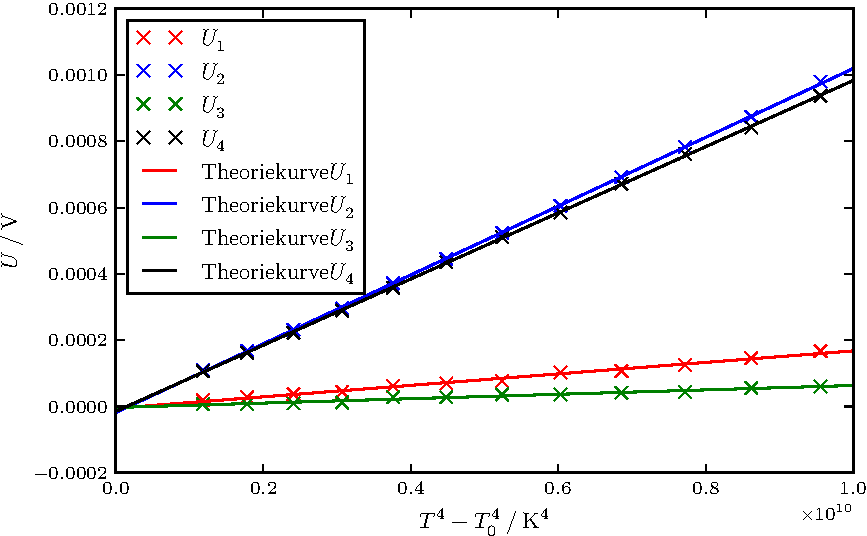
\includegraphics{plot.pdf}
%  \caption{Plot.}
%  \label{fig:plot}
%\end{figure}
%
%\begin{table}
%  \centering
%  \caption{Beispieltabelle}
%  \label{tab:tabelle_beispiel}
%  \sisetup{table-format=1.2}
%  \begin{tabular}{c c}
%    \toprule
%    {$a [\si{\second}]$} & {$b [\si{\kelvin}]$}\\
%    \midrule
%    1.0000  & 11.00 \\
2.0000  & 12.00 \\
3.0000  & 13.00 \\
4.0000  & 14.00 \\
5.0000  & 15.00 \\
6.0000  & 16.00 \\
7.0000  & 17.00 \\
8.0000  & 18.00 \\
9.0000  & 19.00 \\
10.0000 & 20.00 \\

%    \bottomrule
%  \end{tabular}
%\end{table}
%
%Es ergibt sich
%\begin{align}
%  a &= (0 \pm 0) ~ \si{\joule\per\kelvin\per\gram}
 \\
%\end{align}
%
